%------------------------------------------------------------------------------
% Template dos artigos da Revista LUPS
%------------------------------------------------------------------------------

\documentclass[12pt,a4paper,compsoc]{IEEEtran}
\usepackage[utf8]{inputenc}
\usepackage[brazilian]{babel}
\usepackage[dvips]{graphicx}
\usepackage{epsfig}
\usepackage{amsfonts, color}
\usepackage{subfigure}
\usepackage{eurosym}
\usepackage[T1]{fontenc}
\usepackage{ae}

\usepackage{cite}

% Pacotes adicionais
\usepackage{listings}

%------------------------------------------------------------------------------

\begin{document}

%------------------------------------------------------------------------------
%%%%%%%%%%%%%%%%%%%%%%%%%%%%%%%%%%%%%%%%%%%%%%%%%%%%%%%%%%%%%%%%%%%%%%%%%%%%%%%
% Estas informaes devem ser alteradas pelo editor da revista
\pubid{LABORATORY OF UBIQUITOUS AND PARALLEL SYSTEMS~\copyright~LUPS} 
\renewcommand{\leftmark}{REVISTA~LUPS,~VOL.~2, NO.~1,~DEZEMBRO~2013}
%%%%%%%%%%%%%%%%%%%%%%%%%%%%%%%%%%%%%%%%%%%%%%%%%%%%%%%%%%%%%%%%%%%%%%%%%%%%%%%
%------------------------------------------------------------------------------

% Ttulo e autores do artigo

\title{Explorando Regras para Consciência de Situação em Ubicomp}

\author{Caue Duarte, UFPel; Alexandre Gomes da Costa, UFPel

\IEEEcompsocitemizethanks{\IEEEcompsocthanksitem \textbf{Caue Duarte}: Programa de Pós-Graduao em
 Computação,  Universidade Federal de Pelotas - UFPel, Centro de Desenvolvimento Tecnológigo -
 CDTec.
% Para uma quebra de linha, deve-se utilizar o \protect antes do \\, caso contrrio vai dar erro.
\protect\\ E-mail: e-mailautor1@inf.ufpel.edu.br}

% No caso de mais autores, basta repetir:
\IEEEcompsocitemizethanks{\IEEEcompsocthanksitem \textbf{Alexandre Gomes da Costa}: Programa de
 Pós-Graduao em Computação,  Universidade Federal de Pelotas - UFPel, Centro de Desenvolvimento
 Tecnológigo - CDTec.
\protect\\ E-mail: alexandre.costa@inf.ufpel.edu.br}
}

%--------------------------------------------------------------------------------------------------
% ABSTRACT
%--------------------------------------------------------------------------------------------------
\IEEEcompsoctitleabstractindextext{%
\begin{abstract}
  Técnicas de Consciência de Situação são amplamente utilizadas por diversas áreas dentro das
  Ciências da Computação, normalmente ligadas a consequência dos estudos em consciência de
  contexto, com o diferencial possuir raciocínio agregado. Nesse contexto, buscamos no presente
  trabalho definir principais conceitos referentes a computação ubíqua e consciência de situação
  além de explorar o emprego de sistemas baseados em regras para prover esse raciocínio, explorando
  o emprego de regras em trabalhos de grande porte em computação ubíqua.
\end{abstract}

\begin{IEEEkeywords}
Consciência de Situação, Sistemas baseados em regras, Ubicomp, Computação Pervasiva.
\end{IEEEkeywords}}

\maketitle

%--------------------------------------------------------------------------------------------------
% INTRODUÇÃO
%--------------------------------------------------------------------------------------------------
\section{Introduç\~ao}
  \IEEEPARstart{C}{}om o crescente número de dispositivos móveis e o aumento significativo de seu
  poder de processamento e largura de banda, o paradigma da computação ubíqua proposta por Weiser,
  que previa um aumento nas funcionalidades e na disponibilidade de serviços de computação para os
  usuários finais com um custo de gerenciamento ficando cada vez menor, torna-se cada vez mais
  viável.
  
  Técnicas de Consciência de Situação são amplamente utilizadas por diversas áreas dentro da
  Ciência da Computação, incluindo a Computação Ubíqua. Normalmente ligadas a consequência dos
  estudos em consciência de contexto, com o diferencial possuir raciocínio agregado.
  
  Este trabalho explora o uso de Sistemas Baseados em Regras para prover Consciência de Situação.
  Regras podem ser uma generalização geralmente válida, um princípio regulador, um método para a
  realização de uma determinada operação matemática e obter um certo resultado.
  
  Foram analisados os seguintes projetos Collaborative Context-Aware Service Platform for Pervasive
  Computing (CoCA), WComp, a Middleware for Ubiquitous Computing (WComp), A Rule-Based Platform for
  Situation Management (SCENE) e por fim Framework and Rule- based Language for Facilitating 
  Context-aware Computing using Information Appliances - (Context-Aware rule Description Language -
  CADEL).
  
  O objetivo deste trabalho é apresentar conceitos relacionados a Computação Ubíqua, Consciência de
  Situação, Sistemas Baseados em Regras além de explorar o uso de Regras para prover o raciocínio
  utilizado em Consciência de Situação.
  
  O artigo é descrito como segue: na seção 2 são apresentados conceitos de Computação Ubíqua. A
  seção 3 apresenta um breve resumo de Consciência de Situação. A seção 4 introduz conceitos de
  Sistemas Baseados em Regras e mostra sua utilização em projetos relacionados e finalmente na
  seção 5 são apresentadas as conclusões do trabalho.


%--------------------------------------------------------------------------------------------------
% COMPUTAÇÃO UBÍQUA
%--------------------------------------------------------------------------------------------------
\section{Computação Ubíqua}

  O nome Ubíquo vem do Latim \textit{ubiquu}, que significa estar em todos os locais. Mark Weiser,
  então cientista do Centro de Pesquisa da Xerox, definiu em seu artigo intitulado  \textit{The
  Computer for the 21st Century} o termo Computação Ubíqua como sendo a presença direta e constante
  de serviços de computação na vida dos usuários finais, dividindo a computação entre diversos
  dispositivos conectados entre si. O desafio dos cientistas é tornar real o pensamento de Weiser,
  e consequentemente a ubiquidade na computação, fazendo com que as interfaces se tornem
  transparentes, armazenem informações e aprendam a partir dessas informações. Compartilhar dados,
  informações de forma mais fácil e transparente, esta tecnologia fará parte do processo de
  evolução do ser humano, onde cada vez mais a computação centralizada deixar de ser o único agente
  que o usuário interage e multiplicar-se para usos especializados. A Computação Ubíqua,  não se
  resume apenas pela computação, seu objetivo é integrar totalmente a relação
  computação/periféricos com o usuário tornando-se  invisível, no sentido de a utilizar sem 
  perceber.
  
  A computação, embarcada nos mais diversos computadores, já faz parte da vida das pessoas em maior
  ou menor grau e essa interação juntamente com o número da computadores tente a aumentar,
  tornando-se onipresente na vida do usuário. Para tornar isso possível, busca-se a utilização de
  interfaces naturais, tornando a comunicação com esses dispositivos mais transparente, interagindo
  com o usuário por meio de gestos, fala e visão, por exemplo.
  
  Outra forma de interação é através da computação sensível ao contexto, que através do 
  processamento de dados oriundos dos mais diversos sensores, percebe e interage com a realidade do
  ambiente como por exemplo a movimentação do usuário através de um ambiente monitorado.
  O computador, presente nos mais diversos dispositivos (smartphones, tablets, etc..), possui 
  interfaces de comunicação, e como todas interfaces já consolidadas, tende a se tornar 
  imperceptível, uma extensão dos sentidos humanos. Como exemplo de interfaces podemos citar um
  óculos ou uma bengala, que pelo uso contínuo, o usuário abstrai o utensilio em si, utilizando-o
  de forma transparente, focando apenas na realidade trazida pelo mesmo. Sob esta premissa, o uso
  das interfaces passa a tornar-se inconsciente~\cite{weiser1993}. Nesse contexto as aplicações 
  precisam ``entender'' e se ajustar ao ambiente, através do processamento de informações sobre o
  contexto em que estão inseridas ~\cite{maciel2004}.
  
  Essa nova classe de sistemas computacionais, conscientes ao contexto, abre perspectivas para o
  desenvolvimento de aplicações muito mais ricas, elaboradas e complexas, que exploram a natureza
  dinâmica e a mobilidade do usuário. Um desafio central na programação deste tipo de aplicação é
  possibilitar que as mesmas se adaptem continuamente ao ambiente e permaneçam funcionando mesmo
  quando o indivíduo se movimentar ou trocar de dispositivo ~\cite{GrimmB03, Cac08}.
  
  A Computação Ubíqua é entendida como o terceiro grande paradigma computacional, precedido pelos
  \textit{mainframes} e pela computação pessoal ~\cite{weiser1997}. Com foco em demandas 
  institucionais, hoje atende demandas específicas, os \textit{mainframes}, computadores de grande
  porte, atendem requisições de inúmeros usuários. Já com a computação pessoal, observamos uma
  convergência das máquinas para uso pessoal.
  
  Visualizamos a computação ubíqua como uma rede invisível que permeia o usuário com dispositivos
  inteligentes e que se intercomunicam, aprendem uns com os outros, com o ambiente e tomam
  decisões. Os recursos computacionais devem estar disponíveis ao usuário, promovendo adaptações
  dinâmicas tanto dos serviços quanto aplicações satisfazendo as necessidades do usuário, de 
  maneira mais transparente possível. Considerando esta perspectiva, a Computação Ubíqua constitui
  um ambiente altamente distribuído, heterogêneo, dinâmico, móvel, mutável e com forte interação
  entre homem e máquina ~\cite{Augustin03}.
  
  Um caminho breve para a Computação Ubíqua é a imersão total do usuário nessa rede invisível, não
  só de computadores, \textit{smartphones}, \textit{tablets}, mas de dispositivos comuns, até então
  não associados com computação, como eletrodomésticos ao exemplo das já consolidadas 
  \textit{smartv's}, além de outros tantos como mesas, talheres e até ambientes inteiros. Através
  de estratégias de \textit{cloud computing} (computação em nuvem) interligando esses dispositivos
  por rede, internet, \textit{bluetooth} podem trocar dados, processar informações e executar
  qualquer ação que possa ser interessante do ponto de vista do usuário ou sistema.
  

%--------------------------------------------------------------------------------------------------
% CONSCIÊNCIA DE SITUAÇÃO
%--------------------------------------------------------------------------------------------------
\section{Consciência de Situação}

  % Consciência de Situação - Pirâmide
  % Para referenciar a figura ~\ref{cs-piramide}
  \begin{figure}[ht]
  \centerline{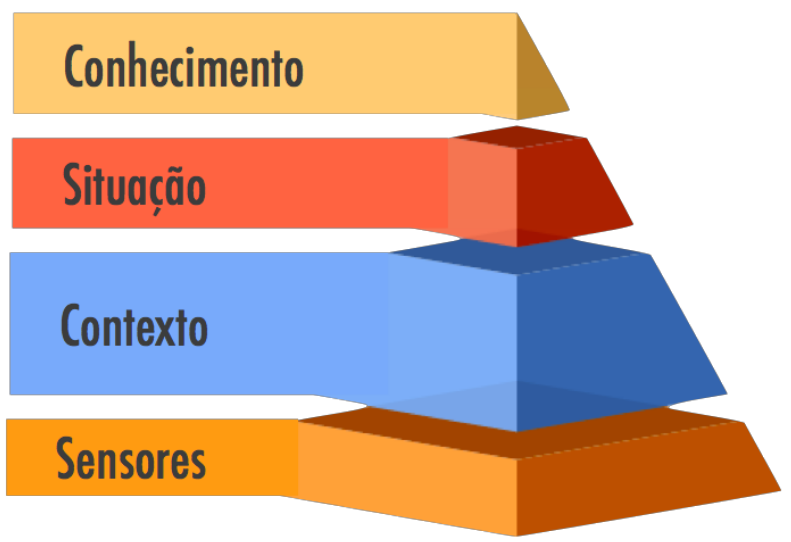
\includegraphics[scale=.20]{imagens/consciencia-de-situacao-piramide}}
  \caption{Consciência de Situação - Pirâmide \cite{almeida2013}}
  \label{cs-piramide}
  \end{figure}

  Consciência de situação é definida como uma interpretação semântica externa dos dados do sensor,
  na área de Computação Ubíqua, \cite{anagnostopoulos2006} define situação como uma 
  particularização da consciência de contexto, onde situações são vistas como contextos logicamente
  ligados.
  
  Então podemos identificar uma pirâmide Fig. \ref{cs-piramide}, onde sensores coletam dados para
  compor contextos e posteriormente serem analisados para identificar possiveis situações.

  Outra definição é que situação consiste de um conjunto de elementos contextuais de interesse 
  instanciados relacionados de forma a prover alguma informação válida em um intervalo de tempo 
  específico, rotulando-os com um nome descritivo. O nome descritivo é uma definição humana de um 
  estado qualquer.
  
  Especificações lógicas de situações são a expressão da correlação dos predicados do contexto. 
  Assim uma situação pode e deve preencher possíveis lacunas de dados de sensores.
  
  Interpretação atribui significado dos dados de sensores com base em estruturas e as relações 
  dentro do mesmo tipo de dados do sensor e entre os diferentes tipos de dados do sensor.
  
  Como na  avaliação de contexto, as questões 5W+1H (quem, o quê, quando, onde, por que e como) são
  levadas em consideração para identificação da situação, sendo que em algumas situações a 
  relevância das perguntas pode mudar.
  
  Conforme a definição de situação apresentada no modelo de Endsley na figura \ref{modelo-endsley} a
  seguir, é introduzida a definição de consciência de situação. Para melhor entendimento do trabalho
  optamos pela seguinte definição de situação: Consciência de situação consiste da percepção e
  compreensão de uma ou mais situações e a projeção de seus efeitos em um futuro próximo
  \cite{endsley1995}. Endsley apresenta três níveis para obtenção de consciência de situação:
  percepção, compreensão e projeção.

  % Modelo de Endsley
  % Para referenciar a figura ~\ref{modelo-endsley}
  \begin{figure*}[ht]
    \centerline{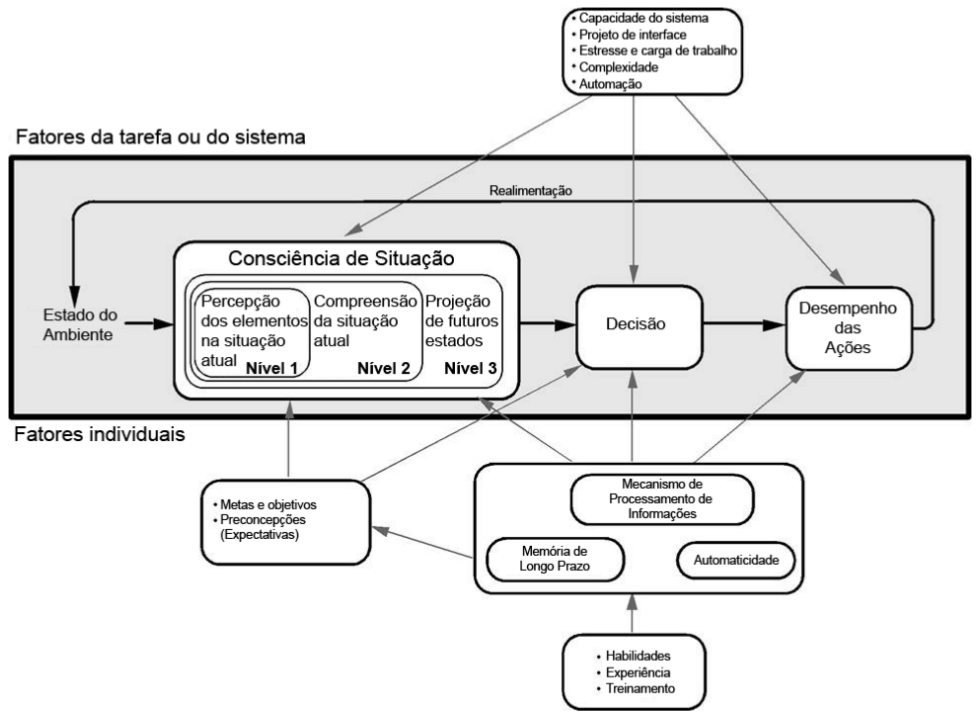
\includegraphics[scale=.35]{imagens/modelo-endsley}}
    \caption{Modelo de Endsley \cite{endsley1995}}
    \label{modelo-endsley}
  \end{figure*}

\subsection{Percepção}

  A percepção (Nível 1)  envolve os processos de monitoramento, detecção e reconhecimento, que
  levam a uma consciência dos elementos situacionais (objetos, eventos, pessoas, sistemas, fatores
  ambientais) e seus estados atuais (locais, condições, formas, ações).


\subsection{Compreensão}

  Além da percepção, é necessário entender todos os elementos e eventos. Então envolvendo uma 
  síntese dos elementos desconexos identificados no primeiro nível através dos processos de 
  reconhecimento de padrões, interpretação e avaliação. Na compressão (Nível 2) integra-se essas
  informações para entender qual a pertinência dessas informações para os objetivos do indivíduo.
  Incluindo o desenvolvimento de uma visão global do ambiente, ou da parte do ambiente que é de 
  interesse do indivíduo. Desempenha um papel fundamental nesta etapa, auxiliando a compreensão do
  ambiente.


\subsection{Projeção}

  O último nível (Nível 3)  é responsável pela previsão de ocorrências futuras, a partir da 
  compreensão dos elementos no ambiente. Ele é alcançado através do conhecimento da situação, da
  dinâmica dos elementos, e da compreensão da situação (níveis 1 e 2), para finalmente projetar e
  verificar se essa informação é pertinente ao estado do sistema em questão.


\subsection{Técnicas de Identificação de Situação}


\subsubsection{Abordagens baseadas em aprendizado}

  Os avanços em tecnologias de sensores impulsionam a implantação de uma ampla gama de sensores,
  que no entanto prejudicam o desempenho das abordagens baseadas em especificações, pois se torna
  inviável apenas usar o conhecimento de especialistas para definir as especificações adequadas
  para situações a partir de um grande número de dados de sensores ruidosos.
  
  Para solucionar essa questão, técnicas de aprendizado de máquina juntamente com técnicas de
  mineração de dados são utilizadas para explorar as relações de associação entre os dados e 
  situações de sensores. Uma grande quantidade de pesquisas tem sido realizadas na área de
  reconhecimento de atividade em ambientes inteligentes, recentemente \cite{knappmeyer2012survey}.
  
  Várias técnicas de situação tem sido utilizadas alcançando bons resultados na identificação de
  situação, embora elas precisem de uma grande quantidade de dados de treinamento para criar um
  modelo e estimar os parâmetros do modelo. Pesquisadores estão motivados com aplicação de técnicas
  de mineração de web para descobrir o conhecimento de senso comum entre as situações e objetos
  minerando os documentos \textit{on-line}, ou seja, o que os objetos são usados em uma determinada 
  atividade humana e como significativo o objeto está em identificar essa atividade.


\subsubsection{Abordagens baseadas em especificações}

  Nos estágios iniciais, a pesquisa de identificação de situação começa quando há alguns sensores,
  cujos dados são fáceis de interpretar e as relações entre os dados e situações de sensores são 
  fáceis de estabelecer.
  
  A pesquisa consiste principalmente em abordagens baseadas em especificações que representam o
  conhecimento especializado nas regras da lógica e aplicar mecanismos de raciocínio para inferir
  situações apropriadas da entrada do sensor de corrente.
  
  No nundo real cada vez mais sensores são implantados em ambientes para uma experiência de longo
  prazo, a incerteza dos dados gerados por esses sensores  começam a ganhar atenção. Para lidar com
  a incerteza, as técnicas baseadas em lógica tradicionais precisam ser incorporados com outras
  técnicas probabilísticas.


%--------------------------------------------------------------------------------------------------
% PROJETOS EM COSCIÊNCIA DE SITUAÇÃO EXPLORANDO REGRAS
%--------------------------------------------------------------------------------------------------
\section{Projetos em Conscincia de Situção Explorando Regras}

  Um dos primeiros e, portanto, mais amplamente desenvolvidos modelos de tomada de decisão são
  sistemas de baseados regras. Seu  desenvolvimento começou na década de 60, mas tornou-se comum
  nos anos 70 e 80.
  
  Regras podem ser  uma generalização geralmente válida, um princípio regulador, um método para a
  realização de uma determinada operação matemática e obter um certo resultado. Exemplos do uso de
  regras:
  
  \textbf{Regras em sistemas especialistas}

  Sua representação assume a forma de pares antecedente-consequente ou instruções if-then, Figura
  \ref{if-then}.;

  % Exemplo de par de instrução if-then
  % Para referenciar a figura ~\ref{if-then}
  \begin{figure}[ht]
    \centerline{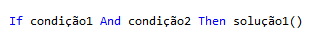
\includegraphics[scale=1]{imagens/if_then}}
    \caption{Exemplo de par de instrução \textit{if-then}}
    \label{if-then}
  \end{figure}
  
  \textbf{Regras na Web Semântica utilizando SW RL}
  
  hasparent(?x1,?x2) $\wedge$ hasBrother(?x2,?x3) $\Rightarrow$ hasUncle(?x1,?x3)

  \textbf{Regras na Computação Ubíqua em ECA-DL}

  Sobre Regra1(p)
  
  Quando Condição(p)
  
  Faça Ação (p, ``mensagem'')


  \textbf{Regras em bancos de dados (regras de consistência)}
  
  Outra forma de definição de regras é através de regras em banco de dados descritas pela consulta SQL
  da Figura \ref{create-table}.
  
  % Exemplo de par de instrução if-then
  % Para referenciar a figura ~\ref{create-table}
  \begin{figure}[ht]
    \centerline{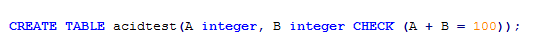
\includegraphics[scale=.6]{imagens/acidtest}}
    \caption{Exemplo de regras utilizando SQL}
    \label{create-table}
  \end{figure}

  Interfaces de configuração de regras de alto nível  Figura \ref{config-cobalto}.

  % Imagem da tela de configuração do Cobalto
  % Para referenciar a figura ~\ref{config-cobalto}
  \begin{figure*}[!ht]
    \centerline{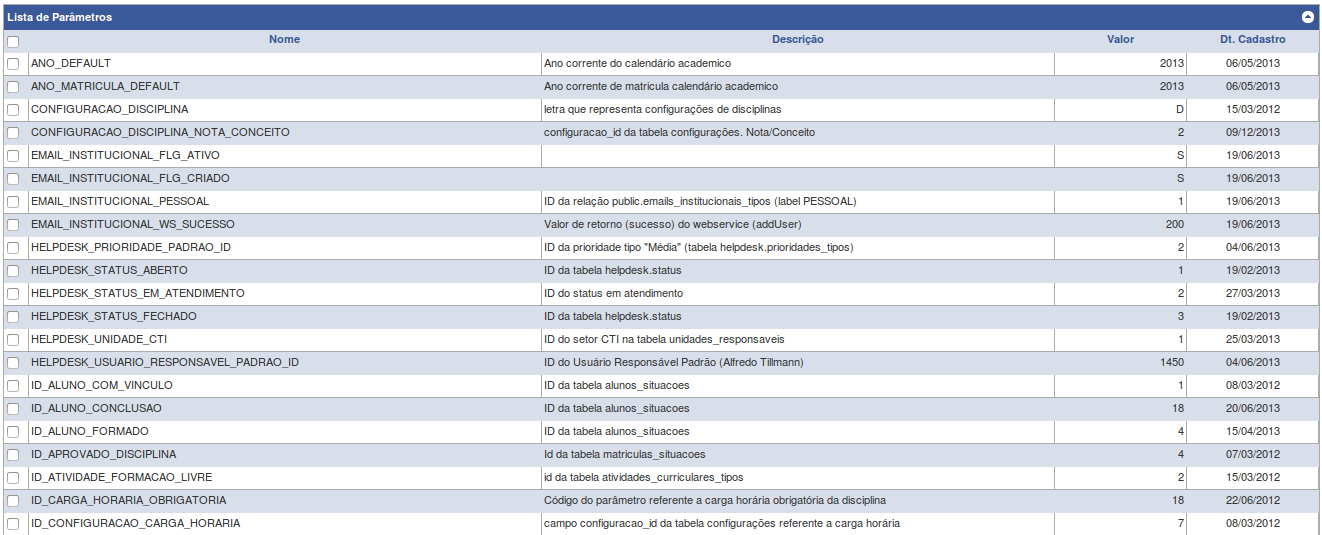
\includegraphics[width=.3\textwidth]{imagens/config-cobalto}}
    \caption{Imagem da tela para configuração do Cobalto}
    \label{config-cobalto}
  \end{figure*}

  Além de suporte para a lógica fuzzy, o método é diferente em termos de,
  
  \begin{enumerate}
    \item Apenas uma regra fica para fornecer a ação;
    \item Arbitragem necessária para determinar qual regra vencerá.
  \end{enumerate}
  
  As vantagens do uso de regras são:

  \begin{itemize}
    \item A existência de base teórica.
    \item Possibilidade de reutilização de regras
    \item Simplicidade de projeto. 
    \item Permite a separação das regras do resto do sistema.
    \item Utilização de plataformas de regras .
    \item Permite adaptação de sistemas \textit{on-the-fly}
    \item Entrega incremental de sistemas
    \item Explanação do processo de inferência
    \item Permite gerar conclusões com grau de incerteza (a partir de premissas imprecisas)
  \end{itemize}
  
  Algumas desvantagens são:

  \begin{itemize}
    \item Desempenho
    \item Pouco relacionamento entre regras (regras se relacionam através do processo de inferência
    apenas)
    \item Podem gerar erros
    \item Dificuldade de lidar com ambiguidades
    \item Regras conflitantes
    \item Base de conhecimento  pode ficar inconsistente e/ou desatualizada  
  \end{itemize}


\subsubsection{Arquitetura de Sistemas Baseados em Regras}

  Cinco componentes básicos compreendem um sistema baseado em regras genéricas,

  \textbf{1. Banco de dados de \textit{Matching}:}

  O banco de dados corresponde ao conjunto de recursos (premissas) que a base de regra usa para
  estabelecer estados. Os recursos são avaliados periodicamente para quaisquer situação contra o
  conteúdo das regras expressas no sistema baseado em regras.

  \textbf{2. Regras de Condição (\textit{Condition-Action Rules}) Uma vez estabelecido o banco de
  dados de fatos a respeito do status dos dados, a regra de condição será expressa conforme exemplo:}

  \begin{lstlisting}
  if condicao1 and condicao2 then
     acao
  \end{lstlisting}

  \textbf{Reescrevendo Regras:}

  Podem existir situações em que uma base de dados é alterada diretamente, sem mais raciocínios,
  tal comportamento é autônomo e geralmente reflete comportamentos NPC mais reativos. Tais casos
  são expressos como regras de reescrita 

  \begin{lstlisting}
  if  condicao1 satisfeita
  and condicao2 satisfeita then
      remove(acao1)
      add(acao2)
  \end{lstlisting}

  \textbf{Encadeamento}
  
  O encadeamento  começa com o conhecimento do objetivo  representado, e em seguida tenta encontrar
  um caminho mínimo através da base de regras para os estados registrados no banco de dados.
  
  \textbf{Arbitragem:}
  
  Geralmente limitar o número de regras para um único caso. Uma das várias heurísticas são 
  geralmente empregadas para esse fim.


\subsection{CoCA - Hybrid Approach to Collaborative Context-Aware Service Platform for Pervasive
 Computing}

  CoCA É um \textit{middleware} baseado em vizinhança, que visa a aquisição e utilização de
  informações de contexto para fornecer serviços, com um modelo de gerenciamento de contexto híbrido
  de grande escalabilidade, formalidade e reutilização.
  
  O Projeto CoCA \cite{ejigu2008hybrid} apresenta uma plataforma colaborativa serviço conscientes
  de contexto baseado no modelo de gestão de contexto híbrido.
  
  O comportamento das aplicações difundidas não dependem apenas em suas interações estaduais e de
  usuários internos, mas também na contextos detectado durante a sua execução. Realizando 
  raciocínio e decisões com base em dados de contexto, semântica contexto e as regras e políticas
  relacionadas, conforme Figura \ref{arquitetura-coca}. Tais dados são organizados em um modelo de
  gestão contexto híbrido, chamado HCOM \cite{ejigu2008hybrid}. Mais tarde, atualizando a ontologia
  com base em modelo de gestão de contexto genérico surge o, GCOM \cite{ejigu2008hybrid}.

  % Arquitetura da plataforma CoCA
  % Referencia da figura ~\ref{arquitetura-coca}
  \begin{figure}[ht]
    \centerline{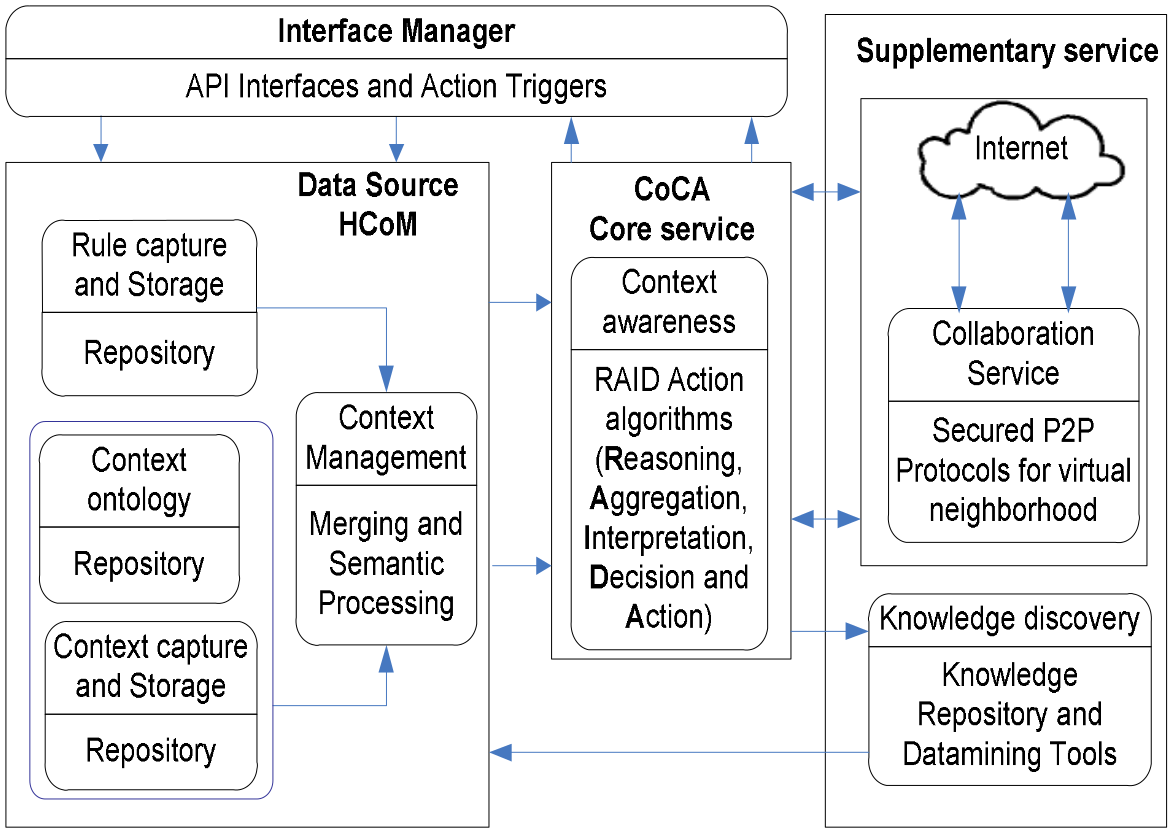
\includegraphics[scale=.2]{imagens/arquitetura-coca}}
    \caption{Arquitetura da plataforma CoCA \cite{ejigu2008hybrid}}
    \label{arquitetura-coca}
  \end{figure}
  
  Apoio à decisão é fornecido de forma proativa ou reativa. É fornecido um suporte à decisão e 
  funcionalidade de ação para minimizar a intervenção do usuário.


\subsection{WComp, a Middleware for Ubiquitous Computing}

  WComp, é um \textit{middleware} para a computação ubíqua. Esse modelo de Middleware é baseado em
  três partes distintas: uma infra-estrutura de software,  um serviço de composição da arquitetura e
  um mecanismo de adaptação.
  
  Para gerenciar o dinamismo e a heterogeneidade das entidades na infra-estrutura de software é
  utilizado WSOAD (\textit{Web Service Oriented Architecture for Device}). As aplicações ubíquas são
  baseadas em um conjunto de serviços Web para dispositivos. Os serviços não são editáveis, logo
  para adicionar novas funcionalidades, uma aplicação tem que ser uma composição de serviços para
  dispositivos.
  
  O WComp utiliza o conceito de Aspectos da Assembleia (AA), baseado em programação orientada a
  aspectos. Eles definem algumas reconfigurações estruturais de um aplicativo que são acionados em
  resposta para eventos da infra-estrutura de software. Eventos informam sobre o aparecimento ou
  desaparecimento de dispositivos da infra-estrutura de software.
  
  Estas regras são compostas e criadas com uma lógica bem definida, no caso de conflito. Eles são
  aplicados em conjuntos de componentes que não são necessariamente conhecidas a priori. Várias
  linguagens e composição de regras podem ser definidas de acordo com o tipo de aplicações nas
  quais eles serão aplicados.


\subsection{SCENE - A Rule-Based Platform for Situation Management}

  Nesse artigo foi proposto uma abordagem para a especificação e realização de detecção de situação
  para uma aplicação de consciência de situação. Foi implementado uma plataforma baseada em regras
  para a gestão de situação (SCENE) que aproveita JBoss Drools adicionando funcionalidade para
  suportar nativamente consciência de situação baseado em regras.
  
  As regras são definidas no Drools por meio de uma linguagem específica de domínio chamado Drools
  Rule Language (DRL). A declaração regra DRL compreende uma condição e um bloco de expressão
  conseqüêntes, respectivamente conhecido como  Left Hand Side (LHS) e Right Hand Side (RHS). A
  regra especifica que quando o determinado conjunto de condições definidas na LHS ocorre, a lista
  de ações na RHS deve ser executado. A LHS é composta de elementos condicionais que podem ser
  combinadas através de operadores lógicos e operadores SET, como  contains e member of. A RHS
  permite a declaração do código que vai ser executado quando as condições definidas na LHS forem
  satisfeitas.
  
  Essas características de situações nos levam aos seguintes requisitos básicos para a nossa
  abordagem de situação:
  \begin{enumerate}
    \item Tipos de situação deve ser definida em tempo de design, e situações instanciar esses
    tipos devem ser detectados em tempo de execução;
    \item Tipos de situação deve ser definido com referência a tipos de entidades, bem como 
    restrições sobre propriedades e relações das entidades;
    \item Propriedades temporais das situações devem ser considerados (tais como o tempo inicial,
    e, para uma situação passado, o tempo final e duração).  
  \end{enumerate}
  
  A fim de atender a estes requisitos, tipos de situação são especificadas no SCENE por meio de 
  aspectos estruturais e comportamentais, que são representados por  \textit{Situation Classes} e
  \textit{Situation Rules}, respectivamente. Cada \textit{Situation Class} definido pelo usuário é
  a especialização da classe pré-definida \textit{SituationType}, que é uma classe abstrata que
  trata das propriedades temporais da situação e características de composição.
  A Figura\ref{situation-classe-fever} ilustra uma \textit{Situation Class}, \textit{Fever}, que
  extends uma classe \textit{SituationType}.
  
  % Situation Class} - textit{Fever}
  % Referencia da figura ~\ref{situation-classe-fever}
  \begin{figure}[ht]
  \centerline{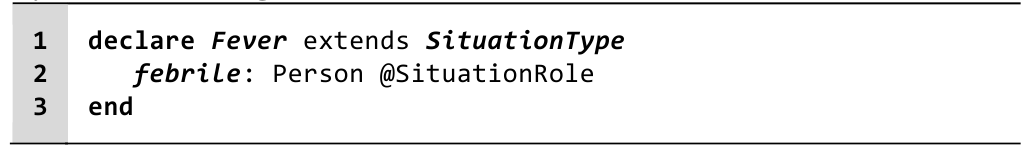
\includegraphics[scale=.25]{imagens/situation-classe-fever}}
  \caption{\textit{Situation Class} - textit{Fever} \cite{pereira2013rule}}
  \label{situation-classe-fever}
  \end{figure}

  Nesse trabalho eles encaram situações como sendo entidades compostas cujos constituintes são
  outras entidades, suas propriedades e as relações em que estão envolvidos. Como exemplo de
  situação podemos ter: ``\textit{John is working}'', ``\textit{John has fever}'', 
  ``\textit{John has had an intermittent fever for the past 6 months}'', 
  ``\textit{John and Paul are outdoors, at a distance of less than 10m from each other}'',
  ``\textit{Bank account number 87346-0 is overdrawn while a suspicious transaction is ongoing}'',
  etc.

  Especificar as situação exige um padrão de regra única seguido de um dialeto de restrição de
  regras padrão Drools. Situações pode ser composta de restrições sobre domínio de entidades, e
  além disso, pode ser composto por situações existentes nelas mesma. Nesse trabalho foram
  abordados aspectos temporais das aplicações, e foi incluído operadores para relacionar situações
  baseadas em seus aspectos temporais. A detecção é baseada em regras, e é implantado um mecanismo
  de regras maduro e eficiente e uma complexa tecnologia de processamento de eventos disponíveis
  para uso. A plataforma gerencia situações através da implementação de situações de controle do
  ciclo de vida, como a ativação da situação, a manutenção do estado e desativação. Não foi
  avaliado o desempenho da detecção da situação, mas esta em curso e por experiência em trabalhos
  anteriores é esperado que o desempenho da detecção de situação seja adequada para a maioria das
  aplicações.


\subsection{CADEL - Framework and Rule-based Language for Facilitating Context-aware Computing
 using Information Appliances}

  Recentemente, computação consciente do contexto, utilizando aparelhos de informação é um dos
  tópicos de pesquisa mais importantes. Em sistemas de computação consciente de contexto, os
  dispositivos são controlados automaticamente com base no contexto atual obtido a partir de vários
  sensores, como posição do usuário, temperatura ambiente e assim por diante. A fim de fazer com
  que os sistemas sensíveis ao contexto funcionem corretamente, é preciso identificar o contexto
  atual do ambiente e para recuperar as regras que podem ser executadas no contexto. Como técnicas
  para descobrir os dispositivos específicos em um ambiente ubíquo.
  
  Mesmo com essas técnicas, a fim de fazer vários dispositivos trabalharem cooperativamente com base
  no contexto, um cenário de como usuário deseja controlar esses dispositivos, deve ser especificado
  com antecedência. Em um cenário, as regras que consistem em condições de sensores e ações de
  dispositivos são descritos. Para especificar cada regra corretamente, é necessário escolher com
  cuidado o conjunto de sensores e dispositivos que o usuário deseja controlar.
  
  Assim, os usuários têm que estarem familiarizados com as suas funcionalidades. No entanto, seria
  muito difícil para os usuários em uma casa comum descrever um cenário viável para fazer o sistema
  funcionar em seus caminhos esperados. Além disso, em um ambiente familiar, vários usuários podem
  querer controlar o mesmo dispositivo em simultâneo de diferentes maneiras.
  
  No artigo desta seção, foi proposto um quadro para permitir que todos possam facilmente descrever
  cenários para sistemas de computação consciente do contexto, incluindo vários aparelhos de
  informação e sensores. A estrutura apresenta do presente trabalho relacionado facilita
  personalização de dispositivos, especificação intuitivo de regras e verificação de consistência e de
  detecção de conflito em várias regras.
  
  Para os fins acima, foi definido uma linguagem chamada CADEL (Context-Aware Linguagem de descrição
  de regras) para especificar regras. O CADEL tem sintaxe e semântica para linguagens naturais
  semelhantes e usuários domésticos comuns pode especificar regras de forma intuitiva. No CADEL, cada
  usuário pode definir novas palavras (por exemplo, \textit{hot-and-stuffy}) para indicar contextos
  específicos detectados a partir de vários sensores.
  
  A estrutura oferece uma função de orientação aos usuários durante a descrição da regra, com o qual
  os usuários podem recuperar os sensores e dispositivos próximos através da GUI e obter as 
  informações, tais como as ações permitidas de um dispositivo e o valor de um sensor. 
  Consequentemente, os usuários podem facilmente especificar uma regra de utilização da informação
  obtida.
  
  O quadro fornece um mecanismo para detectar automaticamente um conflito entre várias regras, o que
  acontece quando as condições de várias regras mantidas ao mesmo tempo executam ações diferentes para
  o mesmo dispositivo. A fim de evitar inconsistências devido a um conflito, foi especificado a
  prioridade entre essas regras conflitantes. Quando uma nova regra é registrada, o quadro verifica se
  há conflitos de regras com as regras vigentes. Se ele entra em conflito, o quadro solicita aos 
  usuários para especificar a prioridade entre as regras. Os usuários podem anexar um contexto 
  específico para a priorizar de modo que a prioridade só funciona no contexto.
  
  Tem sido implementado um protótipo de sistema do quadro proposto em um PC usando UPnP, que
  avaliou o desempenho do sistema em termos de tempo de resposta de recuperação do
  sensor/dispositivo e detecção de conflitos ao longo de várias regras. Através de experimentos,
  foi confirmamos que a implementação do protótipo alcança um desempenho praticamente suficiente
  para executar essas operações.


%------------------------------------------------------------------------------
\section{Considerações Finais}

  O objetivo deste trabalho, além de definir os principais conceitos de computação ubíqua e 
  consciência de situação, foi também aprofundar o estudo do uso de regras em grandes projetos de
  computação ubíqua.
  
  O uso de regras, pelas suas características, tem se mostrado oportuno, sendo explorada de 
  recentemente por grandes projetos de Ubicomp. Pois em diversas situações as vantagens do emprego
  do uso de regras superam suas desvantagens. Neste trabalho foram estudados quatro projetos
  relacionados com a área de computação ubíqua. CoCA realiza raciocínio e decisões com base em 
  dados de contexto, semântica contexto e as regras e políticas relacionadas. O WComp utiliza
  regras para reconfigurações estruturais de um aplicativo que são acionados em resposta para
  eventos da infra-estrutura de software. SCENE utiliza uma plataforma baseada em regras para a
  gestão de situação que aproveita JBoss Drools adicionando funcionalidade para suportar 
  nativamente consciência de situação baseado em regras. No CADEL as regras consistem em condições
  de sensores e ações de dispositivos descritos.

%------------------------------------------------------------------------------
\bibliographystyle{unsrt}
\bibliography{BIBFile}


%------------------------------------------------------------------------------
%Biografia dos autores

\begin{IEEEbiography}[{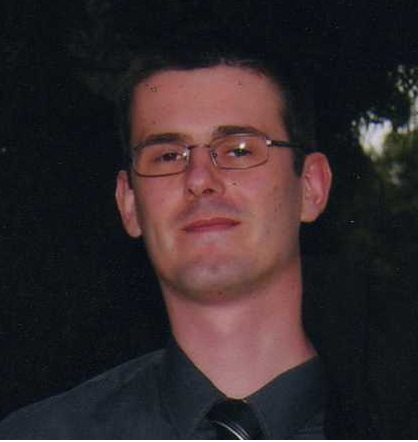
\includegraphics[width=1in, height=1.25in, clip, keepaspectratio] 
  {imagens/fotocaue}}]{Caue Duarte}

  Possui graduação em Análise e Desenvolvimento de Sistemas pela Universidade Norte do Paraná.
  Técnico em Eletrônica pelo Instituto Federal Sul-Rio-grandense. Possui Pós-Graduação com Enfase
  em Educação à Distância , atualmente é mestrando no Programa de Pós-Graduação em Computação da
  UFPel (Mestrado em Ciência da Computação). Atua como técnico em Sistemas de Informação da
  Universidade Federal de Pelotas, onde desenvolve sistemas, interfaces e realiza modelagem de
  sistemas e banco de dados. Também atua como professor do Instituto Educacional Dimensão, no
  curso de Análise de Sistemas. 
% Quanto a foto, no deve ser de corpo inteiro (deve ser similar ao avatar de exemplo) e convertida
% em escala de cinza.
\end{IEEEbiography}

\begin{IEEEbiography}[{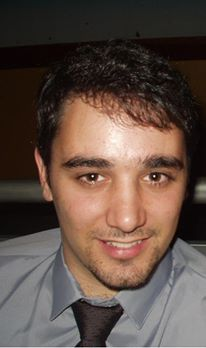
\includegraphics[width=1in, height=1.25in, clip, keepaspectratio]
  {imagens/fotoalexandre}}]{Alexandre Gomes da Costa}

  Aluno Especial do Programa de Pós-Graduação em Computação da Universidade Federal de Pelotas. Possui
  Bacharel em Ciência da Computação (2008) pela Universidade Federal de Pelotas.
  
% Quanto a foto, no deve ser de corpo inteiro (deve ser similar ao avatar de exemplo) e convertida
% em escala de cinza.
\end{IEEEbiography}

\end{document}


